\recipe{Murray's Pembroke Shakshuka}
\label{recipe:murrays_pembroke_shakshuka}
\makes{3 portions}
\worktime{\SI{10} \minute}
\totaltime{\SI{40} \minute}
\source{Original recipe}

\begin{ingredients}
  \item 1 Onion, chopped
  \item 1 Green bell pepper, chopped
  \item Garlic, 2 cloves, finely chopped
  \item Chopped tomatoes, $2 \times $ \SI{400}{\gram} tins
  \item Extra virgin olive oil, \SI{1}{\tablespoon}
  \item Paprika, \SI{1}{\teaspoon}
  \item Ground cumin, \SI{1}{\teaspoon}
  \item Chilli powder, \qty{0.5}{\teaspoon}
  \item Coriander, \SI{1}{\teaspoon}
  \item Red pepper flakes, \qty{0.5}{\teaspoon}
  \item Salt, to taste
  \item Eggs, 6 large

  \ingroup{To Serve}
  \item Fresh parsley, 1 handful, chopped
  \item Fresh mint, 1 handful, chopped
  \item Feta, \SI{50}{\gram}, crumbled
  \item Sourdough bread, to serve
  \item Orange juice or mimosa, optional
\end{ingredients}

\begin{method}
  Heat \SI{1}{\tablespoon} extra virgin olive oil in a large skillet over medium heat. Add the chopped onion, green bell pepper, and garlic and sauté for \SI{5}{\minute}, stirring occasionally, until the vegetables are tender.

  Season with salt, \SI{1}{\teaspoon} coriander, \SI{1}{\teaspoon} paprika, \SI{1}{\teaspoon} cumin, \qty{0.5}{\teaspoon} chilli powder, and \qty{0.5}{\teaspoon} red pepper flakes. Stir and cook for a further \SI{1}{\minute}.

  Add the \SI{800}{\gram} chopped tomatoes and bring the mixture to a gentle boil. Cover and simmer over low heat for \SI{15}{\minute}. Remove the lid and cook for a further \SI{5}{\minute}, or until the sauce has thickened.

  Crack 6 eggs into 6 evenly spaced wells in the tomato sauce.

  Cover the skillet and cook over medium-low heat for \SI{5}-\SI{8}{\minute}, until the egg whites have set but the yolks remain slightly runny.

  Scatter over the chopped parsley, mint, and crumbled feta. Serve immediately with sourdough bread.
\end{method}

\begin{figure}[h]
  \centering
  
  \begin{minipage}{0.48\linewidth}
  	\centering
	\begin{tikzpicture}
    		% Save the image at 110% scale
	    \sbox0{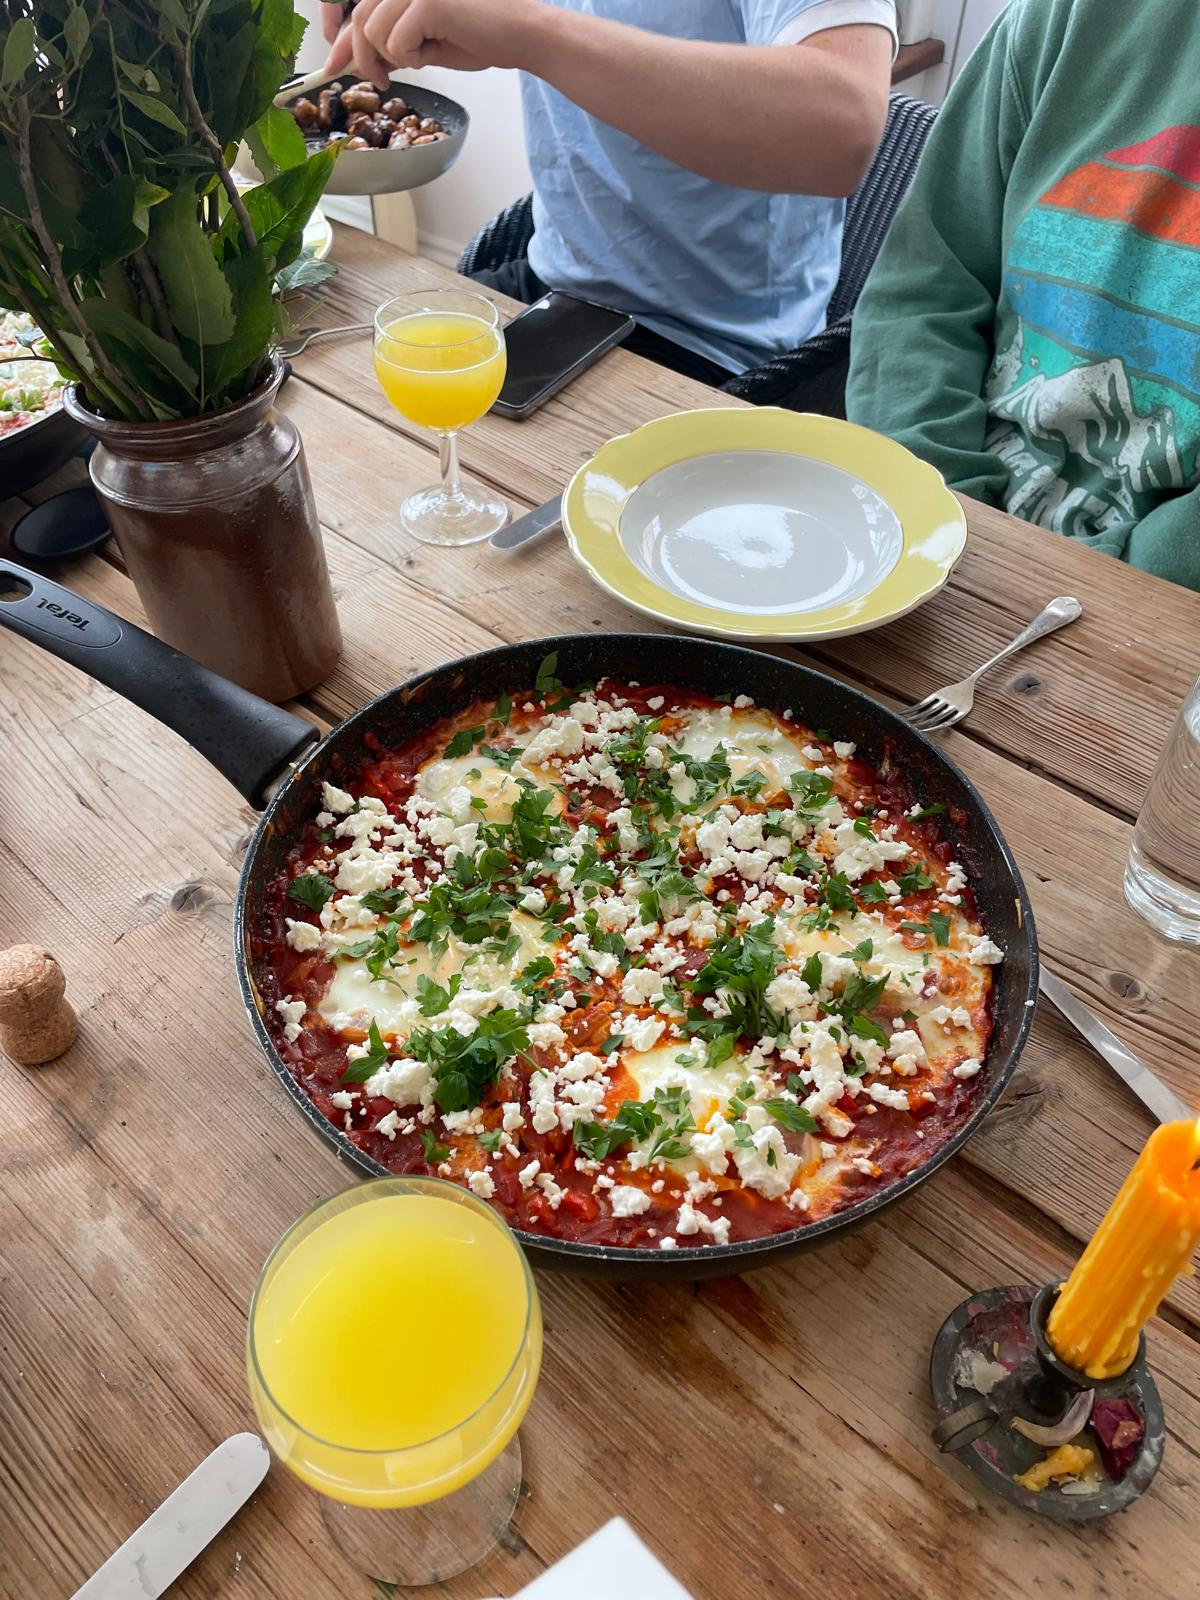
\includegraphics[width=\linewidth]{images/shakshuka.jpg}}%

	    % Landscape clipping rectangle
	    \path[
    	    clip,
    	    	rounded corners=0.5cm
	    ] (0,0) rectangle (\linewidth,0.7\linewidth);

	    	% Ce	nter the zoomed image inside the landscape crop
    		\node[
    		    inner sep=0pt,
        		outer sep=0pt,
	        anchor=center
    		] at (0.5\linewidth, 0.55\linewidth) {\usebox0};
	\end{tikzpicture}
  \end{minipage}
  \hfill
  \begin{minipage}{0.48\linewidth}
  	\centering
	\begin{tikzpicture}
    		% Save the image at 110% scale
	    \sbox0{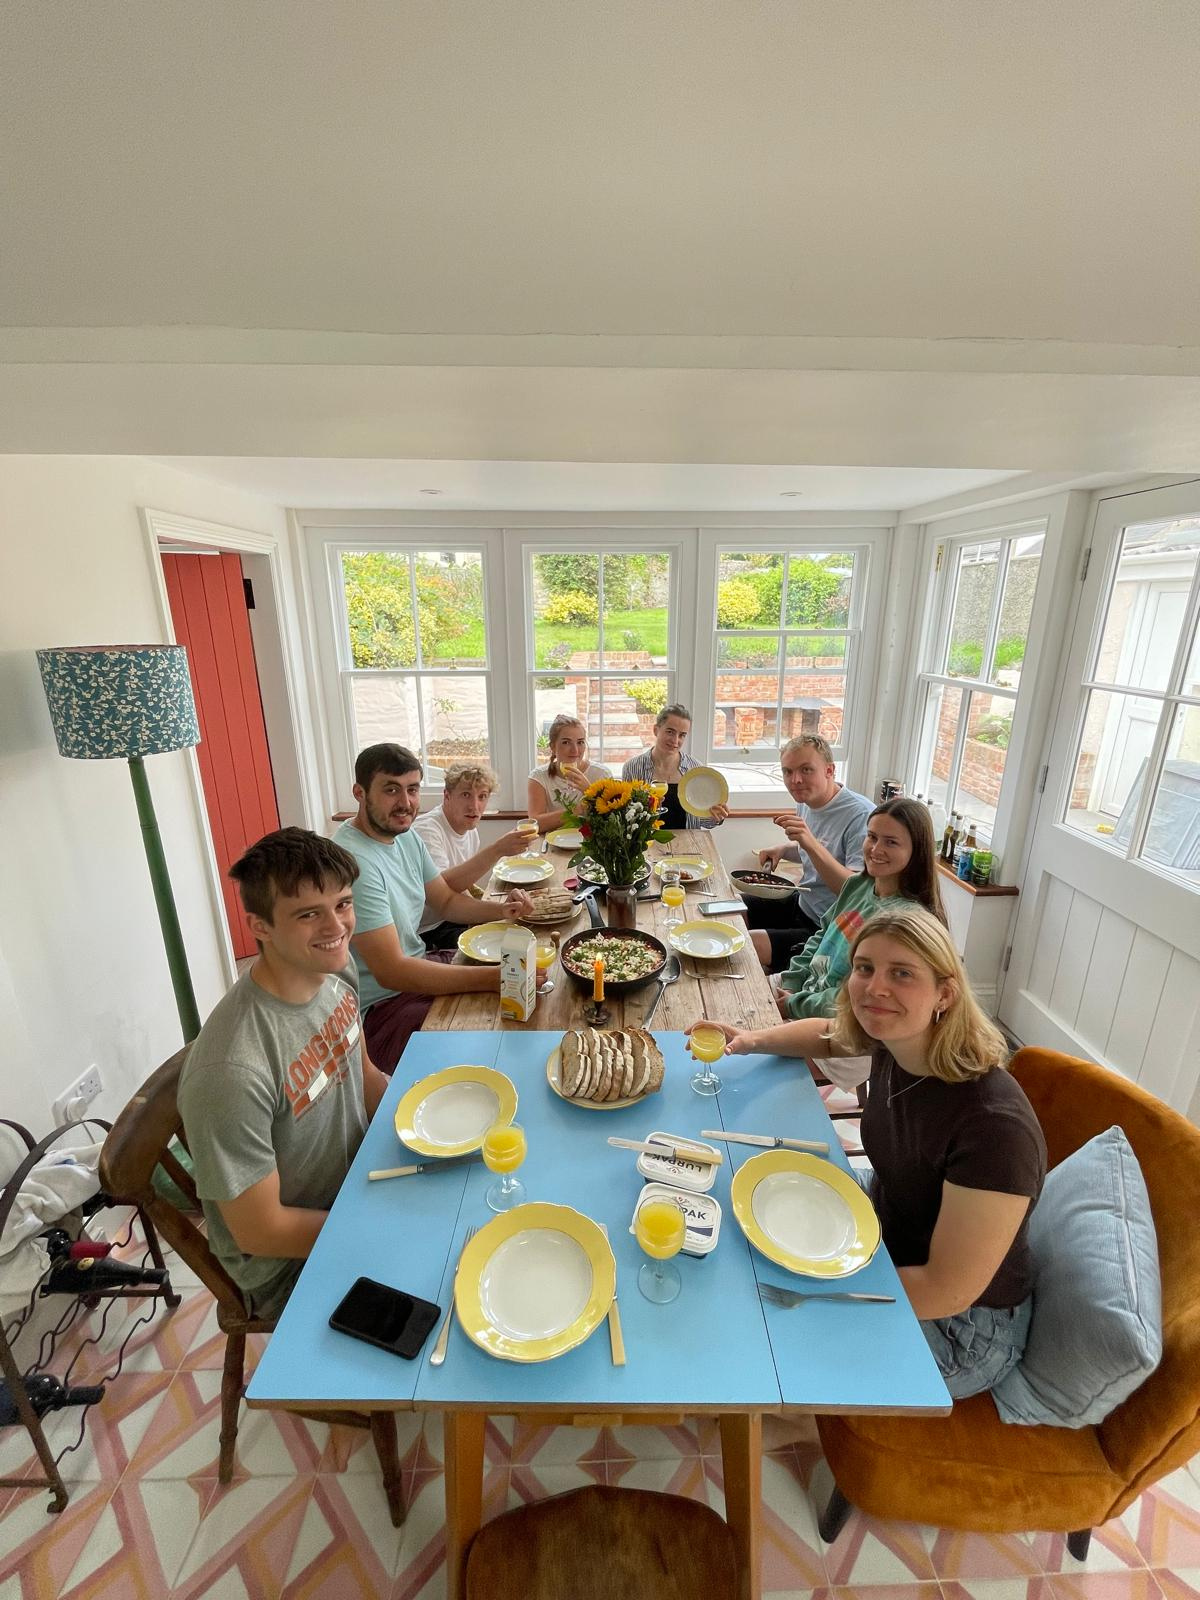
\includegraphics[width=\linewidth]{images/shakshuka2.jpg}}%

	    % Landscape clipping rectangle
	    \path[
    	    clip,
    	    	rounded corners=0.5cm
	    ] (0,0) rectangle (\linewidth,0.56\linewidth);

	    	% Ce	nter the zoomed image inside the landscape crop
    		\node[
    		    inner sep=0pt,
        		outer sep=0pt,
	        anchor=center
    		] at (0.5\linewidth, 0.45\linewidth) {\usebox0};
	\end{tikzpicture}
  \end{minipage}
\end{figure}

\begin{notes}
Serve with homemade sourdough. Orange juice or a mimosa makes a good accompaniment.
\end{notes}